\documentclass{article}

\usepackage{graphicx}
\usepackage{tikz}
\usepackage{tikzsymbols}
\usetikzlibrary{calc,patterns,shapes.geometric}
\pagestyle{empty}
\usepackage[margin=0pt]{geometry}
\geometry{papersize={14in,12in}}

\def\centerarc[#1](#2)(#3:#4:#5){\draw[#1] ($(#2)+({#5*cos(#3)},{#5*sin(#3)})$) arc (#3:#4:#5);}

\begin{document}
	\begin{figure}
		\centering
		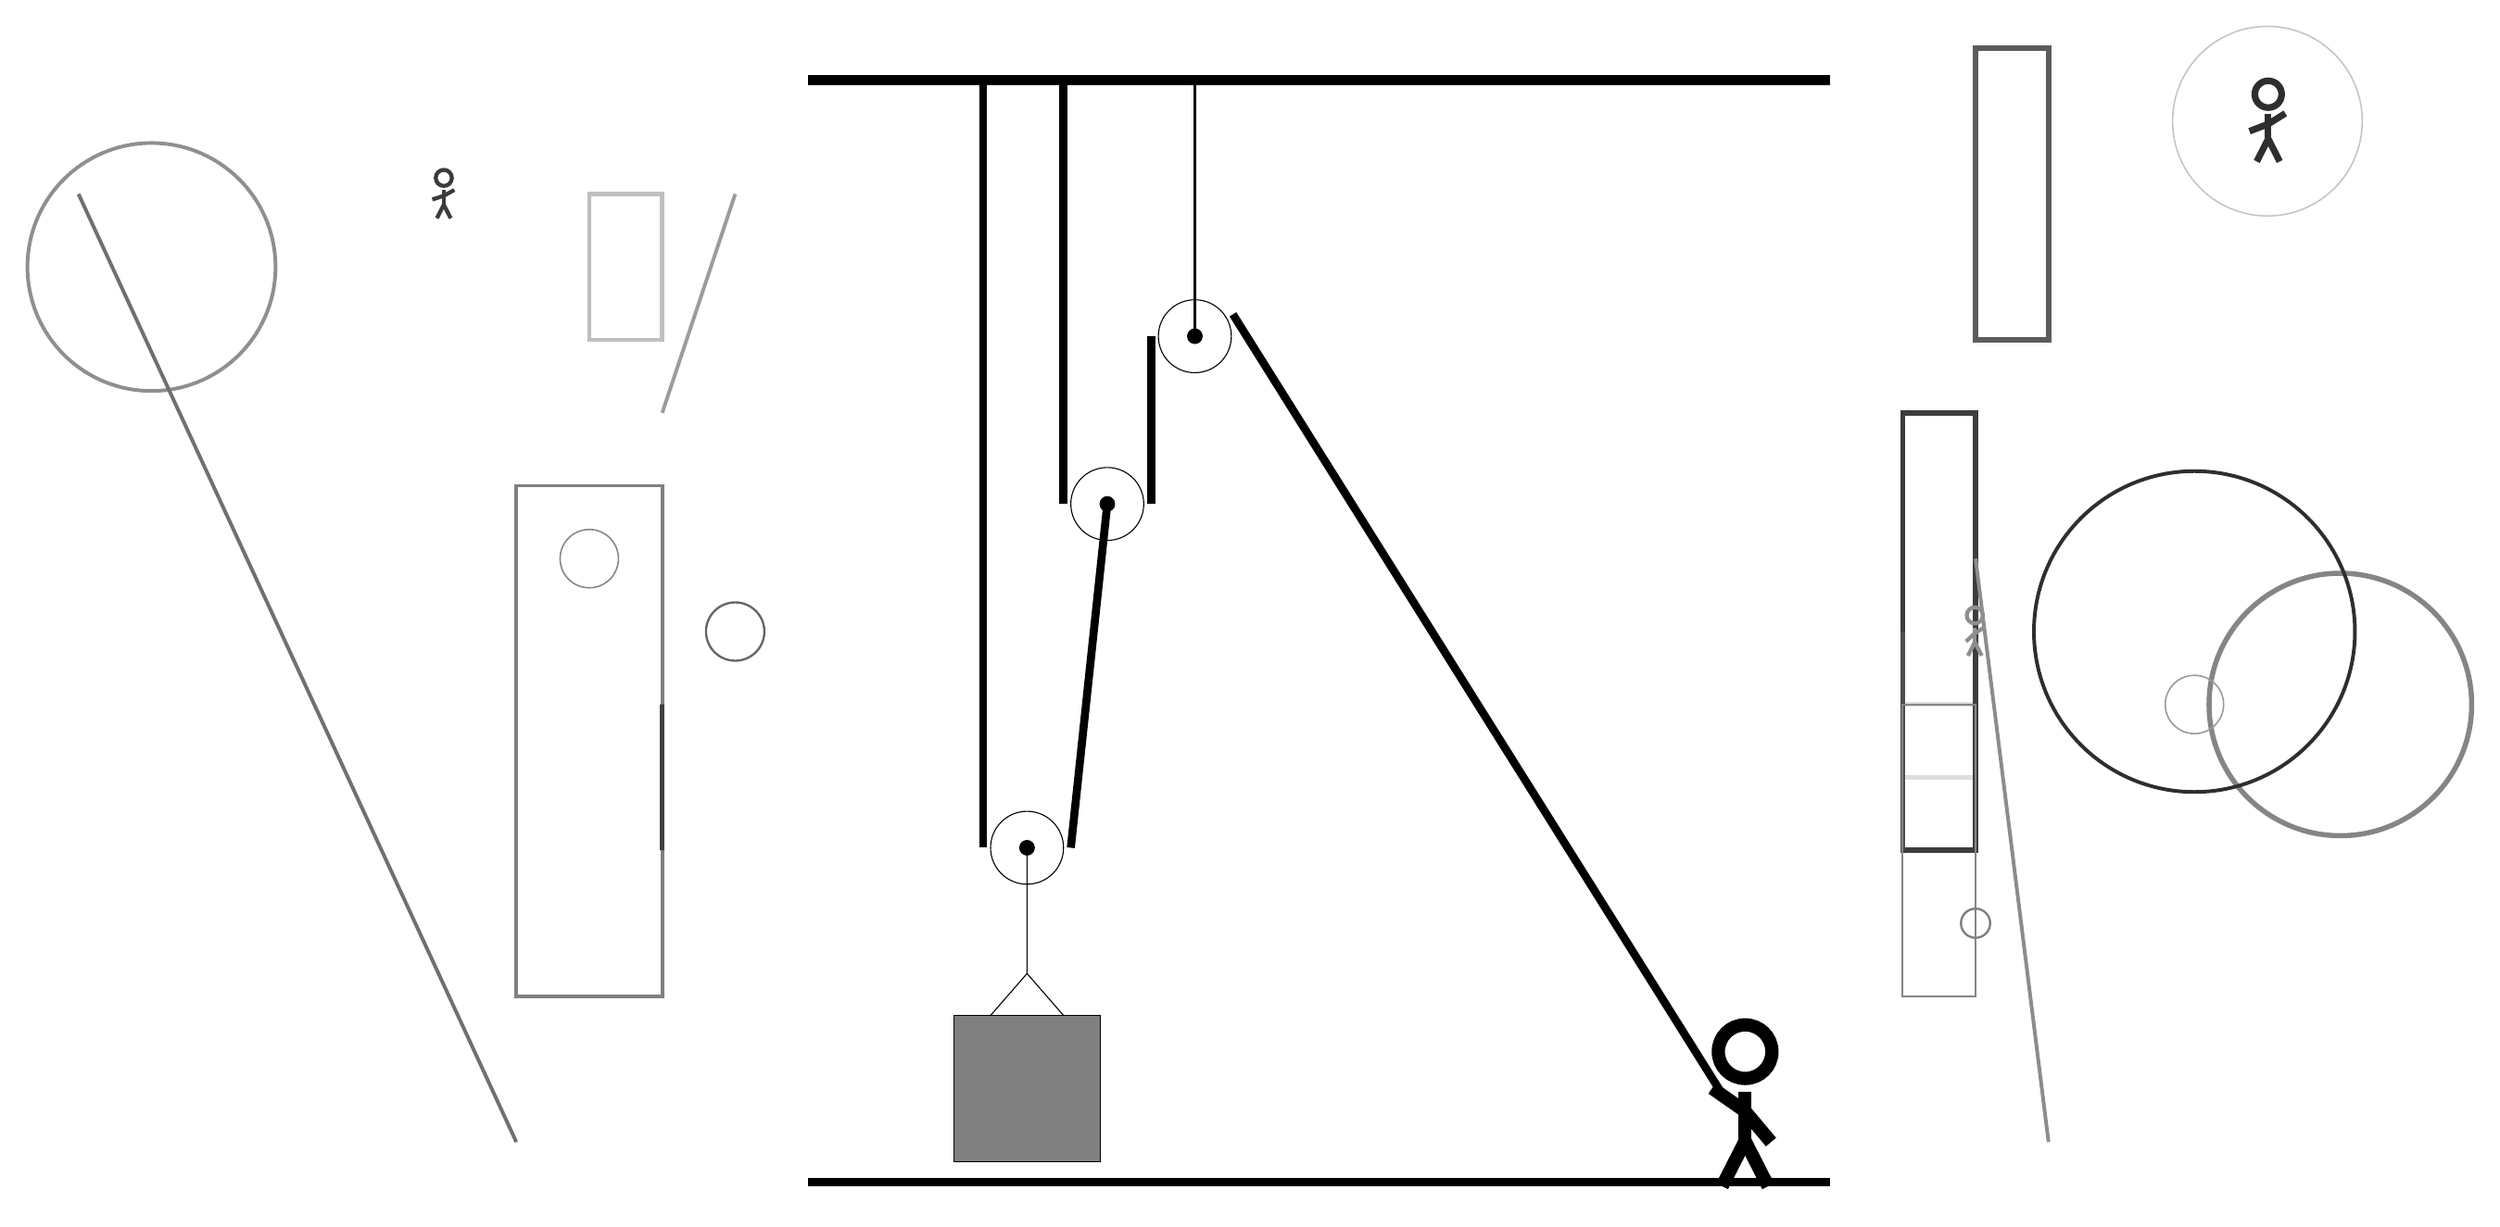
\begin{tikzpicture}
			%%%%% START %%%%%
			
			\draw[fill=black] (-2, 11.5) rectangle (12, 11.625);
			
			\draw (1, 1.035) circle (0.5);
			\draw[fill=black] (1, 1.035) circle (0.1);
			
			\draw (2.1, 5.75) circle (0.5);
			\draw[fill=black] (2.1, 5.75) circle (0.1);
			
			\draw (3.3, 8.05) circle (0.5);
			\draw[fill=black] (3.3, 8.05) circle (0.1);
			\draw[thick] (3.3, 8.05) -- (3.3, 11.5);
			
			\draw (1, 1.035) -- (1, -0.69) -- (0.5, -1.265) -- (1.5, -1.265) -- (1, -0.69);
			\draw[fill=black!50] (0, -1.265) rectangle (2, -3.265);
			
			\draw[line width=1.1mm] (0.4, 11.5) -- (0.4, 1.035);
			\centerarc[line width=1.1mm](1, 1.035)(180:360:0.6);
			\draw[line width=1.1mm](1.6, 1.035) -- (2.1, 5.75);
			\draw[line width=1.1mm] (1.5, 11.5) -- (1.5, 5.75);
			\centerarc[line width=1.1mm](2.1, 5.75)(180:360:0.6);
			\draw[line width=1.1mm](2.7, 5.75) -- (2.7, 8.05);
			\centerarc[line width=1.1mm](3.3, 8.05)(30:180:0.6);
			\draw[line width=1.1mm] (3.822, 8.35) -- (10.5, -2.3);
			
			\node at (10.8, -2.5) {\Strichmaxerl[10][-35][-50]};
			
			\draw[line width=0.7mm, color=black!13] (14, 2) rectangle (13, 3);
			
			\draw[line width=0.7mm, color=black!76] (13, 1) rectangle (14, 7);
			\draw [line width=0.7mm, color=black!48](19, 3) circle (1.8);
			\draw [line width=0.2mm, color=black!23](18, 11) circle (1.3);
			
			\draw[line width=0.5mm, color=black!50] (-4, 6) rectangle (-6, -1);
			
			\draw [line width=0.2mm, color=black!40](17, 3) circle (0.4);
			
			\node[line width=0.5mm, color=black!77] at (-7, 10) {\Strichmaxerl[3][18][29]};
			
			\draw[line width=0.5mm, color=black!45](15, -3) -- (14, 5);
			\draw[line width=0.5mm, color=black!39](-3, 10) -- (-4, 7);
			
			\node[line width=0.4mm, color=black!44] at (14, 4) {\Strichmaxerl[3][43][32]};
			
			\draw[line width=0.6mm, color=black!25] (-4, 8) rectangle (-5, 10);
			\draw [line width=0.3mm, color=black!51](14, 0) circle (0.2);
			\draw [line width=0.5mm, color=black!82](17, 4) circle (2.2);
			\draw [line width=0.3mm, color=black!60](-3, 4) circle (0.4);
			\draw [line width=0.2mm, color=black!48](-5, 5) circle (0.4);
			\node[line width=0.2mm, color=black!82] at (18, 11) {\Strichmaxerl[5][21][32]};
			\draw[line width=0.7mm, color=black!64] (14, 8) rectangle (15, 12);
			\draw[line width=0.6mm, color=black!70] (13, 4) rectangle (13, 1);
			\draw [line width=0.5mm, color=black!44](-11, 9) circle (1.7);
			\draw[line width=0.5mm, color=black!56](-6, -3) -- (-12, 10);
			\draw[line width=0.7mm, color=black!75] (-4, 1) rectangle (-4, 3);
			
			\draw[line width=0.3mm, color=black!48] (14, -1) rectangle (13, 3);
			
			\draw[fill=black] (-2, -3.5) rectangle (12, -3.6);
			
			%%%%% END %%%%%
		\end{tikzpicture}
	\end{figure}	
\end{document}